\documentclass{article}
\usepackage{blindtext}
\usepackage{graphicx}
\usepackage{gensymb}
\usepackage{array}
\usepackage[utf8]{inputenc}
\graphicspath{ {Images/} }
\usepackage{biblatex}
\addbibresource{Test1.bib}

\title{Hot Chips}
\author{Gavin Barnett}
\date{\today}

\begin{document}
\maketitle
	\begin{figure}[h]
		\centering
		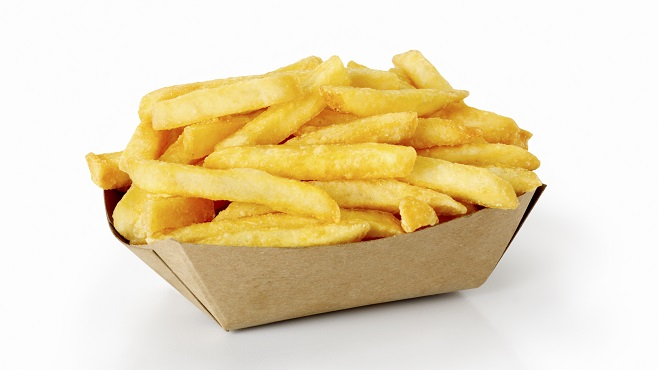
\includegraphics[scale=2.3]{Hot-chips-Getty}
		\caption{Hot-Chips}
	\end{figure}
\begin{abstract}
Random readings and rambling on the effects of high temperatures on electronic devices. 
Also getting use to using LaTeX.

\end{abstract}
\maketitle

\newpage

\tableofcontents

\newpage

\section{Introduction}

\newpage


\section{IC Packaging Considerations}
	\begin{figure}[h]
		\centering
		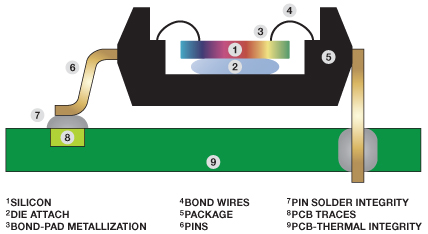
\includegraphics[scale=1]{Package_Breakdown}
		\caption{Packaging}
		\label{fig:packaging}
	\end{figure}
	
	
	\subsection{Silicon}
		\subsubsection{Crystalline structure failure}
		\subsubsection{Hot Carrier Injection (HCI)}
		\subsubsection{Negative Bias Temperature Instability (NBTI)}
	
	\subsection{Die Attach}
		\subsubsection{Coefficient of Thermal Expansion(CTE)}
	
	\subsection{Wire Bond/ Bond-Pad Metallization}
		\subsubsection{Inter-Metallic Compound (IMC) Growth}
		\subsubsection{Diffusion (Kirkendall Effect)}
		\subsubsection{Corrosion}
	
	\subsection{Package}
		\subsubsection{Glass-Transition Temperature (Tg)}
		\subsubsection{Coefficient of Thermal Expansion(CTE)}
		\subsubsection{Hermetic Ceramic Packages}
		\subsubsection{High-Temperature Multichip Modules}
	
	\subsection{Pins}
		\subsubsection{Through Hole}
		\subsection{Gull-Wing SMT}
		\subsubsection{BGA}
	
	\subsection{Pin Solder Integrity}
		% Ref: (http://www.logwell.com/tech/servtips/solder.html)
		% Ref2: (http://www.logwell.com/tech/app_notes/Temps.pdf)
		% Ref3: (http://store.curiousinventor.com/guides/how_to_solder/kind_of_solder)
		% Ref4 : (see the graph here - https://www.thegearpage.net/board/index.php?threads/lead-free-solder.1335612/)
		Solder is a fusible metal alloy used to connect devices and wire to the PWA.
		Typical melting points for solder are around 180-190\degree although this varies with solder alloy. 
		For high temperature electronics it is important to consider the melting point of solder used, including that on BGA devices.
				% Ref: http://ostec-materials.ru/upload/iblock/714/71418246221db5e84a71e8973b38f94e.pdf
				
		Solder is made of a a number of elements, typically these include:
		\begin{itemize}
			\item Tin (Sn)
			\item Lead (Pb)
			\item Antimony (Sb)
			\item Bismuth (Bi)
			\item Indium (In)
			\item Gold (Au)
			\item Silver (Ag)
			\item Zinc (Zn)
			\item Copper (Cu)
		\end{itemize}
		
		\subsubsection{Eutectic}
		A material is said to be Eutectic if its melting point is the same as its freezing point. 
		This can also be phrased has having the same liquidus (melting) and solidus (freezing) temperature.
		
		Non-eutectic alloys go through a cooling phase (or melting range) where solid particles are flowing within a liquid. Any movement of a cooling non-eutectic alloy in this "pasty state" can cause poor joints to form on the work piece.  		
	
		\subsubsection{Tin/lead solder alloys}	 
		 Typical melting point around 180\degree
		\begin{center}
 			\begin{tabular}{| m{10em} | m{5em}| m{17em} | } 
 			\hline
 			\textbf{Composition} & \textbf{Melting Range} & \textbf{Description} \\ [0.5ex] 
 			\hline\hline
 			63Sn/37Pb & 183\degree & Eutectic  \\ 
 			\hline
 			60Sn/40Pb & 183-188\degree & Classic solder \\
 			\hline
 			62Sn/36Pb/2Ag & 179\degree & Very common and strongest tin/lead solder \\
 			\hline
 			90Pb/10Sn & 275-302\degree & Increased lead increases melting point \\
 			\hline
 			95Pb/5Sn & 308-312\degree & Increased lead increases melting point \\
 			\hline
			\end{tabular}
		\end{center}
The higher temperature, higher lead content solders where used internally within devices to prevent re-flow during PWA assembly.
				
		\subsubsection{Lead-free solder alloys}
		These are typically made up of the SAC alloys Tin (Sn) / Silver (Ag) /Copper (Cu) and are mostly eutectic. 
		Although at high temperatures they tend to dissolve copper. 
		As such the process must be well controlled adding SN/Ag as required.
				
		An alternative alloy of Tin (Sn) / Bismuth (Bi) / Silver (Ag) may be better for wetting and fatigue resistance than SAC.
		Although if combined with lead (Pb) from any devices it can form a lead alloy with melting points as low as 96\degree , which is highly problematic.
		 \begin{center}
 			\begin{tabular}{| m{10em} | m{5em}| m{17em} |} 
 			\hline
 			\textbf{Composition} & \textbf{Melting Range} & \textbf{Description} \\ [0.5ex] 
 			\hline\hline
 			96.5Sn/3.0Ag/0.5Cu & 217-220\degree & Near eutectic. It is the JEITA recommended alloy for wave and reflow soldering \\ 
 			\hline
 			95.6Sn/3.5Ag/0.9Cu & 217\degree & Eutectic. \\ 
 			\hline
 			91.8Sn/4.8Bi/3.4Ag & 211-213\degree & Do not use on lead-containing assemblies \\
 			\hline
			\end{tabular}
		\end{center}
		
		\subsubsection{Low-temperature alloys}
		By adding Indium(In) and Bismuth (Bi) to solder alloys the melting point can be lowered.
		 \begin{center}
 			\begin{tabular}{| m{10em} | m{5em}| m{17em} |} 
 			\hline
 			\textbf{Composition} & \textbf{Melting Range} & \textbf{Description} \\ [0.5ex] 
 			\hline\hline
 			52In/48Sn & 118\degree & Eutectic. \\ 
 			\hline
 			58Bi/42Sn & 138\degree & Eutectic. \\ 
 			\hline
 			80In/15Pb/5Ag & 142-149\degree &  \\
 			\hline
			\end{tabular}
		\end{center}
		
		\subsubsection{High-temperature solder alloys}
		
		
		\subsubsection{Indium-lead for thick gold metallizations}
		
		
		\subsubsection{High Melting Point (HMP) alloys}
	
	\subsection{Printed Wiring Board (PWB)}
		\subsubsection{Glass Transition Temperature (Tg)}
		\subsubsection{De-lamination}
		\subsubsection{Moisture Absorption}

	\subsection{Printed Wiring Assembly (PWA)}
		\subsubsection{Tin-whiskers}
		\subsubsection{Flux residue}
		\subsubsection{Conformal Coating}

\newpage

\section{Passives}
	\subsection{Resistors}
	
	\subsection{Capacitors}
	
	\subsection{Inductors}
	
\newpage

\section{Fault Phenomenon}
	\subsection{Leakage Currents}
	In capacitors the "leakage current" is a small amount of current which flows across the dielectric material. This can also be expressed as a large shunt resistance known as "insulation resistance".
	
	\subsubsection{Dielectric Absorption Currents}
	This is the current required to align the dipoles with the dielectric.
	
	\subsubsection{Quantum Tunnel Effects}


\newpage

\printbibliography

\end{document}
